\chapter{Background and Related Work}
\label{ch:background}

\section{RISC-V RV64I Architecture}
The RISC-V instruction set architecture (ISA) is an open and modular standard designed to promote extensibility, simplicity, and freedom from licensing restrictions~\cite{riscv-spec}.  
The base 64-bit subset, known as RV64I, defines a general-purpose architecture supporting 64-bit integer arithmetic and memory addressing.  
It serves as the foundation for all higher-level RISC-V extensions and implementations.

\subsection{Registers and Data Model}
The RV64I ISA defines 32 general-purpose registers (\texttt{x0--x31}), each 64~bits wide.  
Register \texttt{x0} is hardwired to zero, while \texttt{x1} (\texttt{ra}) holds the return address.  
Registers \texttt{x2} (\texttt{sp}) and \texttt{x3} (\texttt{gp}) serve as the stack pointer and global pointer, respectively.  
The remaining registers are divided between temporary (\texttt{t0--t6}), saved (\texttt{s0--s11}), and argument (\texttt{a0--a7}) registers.  
The architecture uses a little-endian data model and supports naturally aligned accesses to 8-, 16-, 32-, and 64-bit data.

The program counter (\texttt{pc}) is a 64-bit register that stores the address of the next instruction.  
Each instruction is 32 bits wide and aligned to a 4-byte boundary, simplifying instruction fetch and decode stages in hardware.

\subsection{Calling Convention and Program Flow}
The RWU-RV64I processor adheres to the standard RISC-V calling convention.  
Function arguments are passed through registers \texttt{a0--a7}, and return values are stored in \texttt{a0}.  
The stack grows downward from the top of data memory, and all functions preserve the values of callee-saved registers (\texttt{s0--s11}).  
After a system reset, the processor’s program counter starts at address \texttt{0x00000000}, where the startup code (\texttt{\_start}) resides.  
This startup routine initializes memory and transfers control to the user’s \texttt{main()} function.

\subsection{Instruction Formats and Execution Flow}
RISC-V instructions follow six fundamental encoding formats—R, I, S, B, U, and J—each specifying a unique arrangement of opcode, register indices, and immediate fields~\cite{riscv-spec}.  
This regular structure provides a compact and consistent encoding scheme, simplifying both hardware decoding and compiler implementation.  
The details of these formats and their corresponding instruction classes are described in Section~\ref{sec:rv64i_instructions}.

During execution, the RWU-RV64I processor fetches instructions sequentially from instruction memory (IMEM), decodes them through its control unit, and performs arithmetic or memory operations using the arithmetic logic unit (ALU) and data memory (DMEM).  
The architecture follows a Harvard memory model, ensuring that instruction fetch and data access can occur independently and concurrently within a single clock cycle.

\section{RISC-V RV64I Instruction Set}
\label{sec:rv64i_instructions}

The RV64I instruction set constitutes the base integer subset of the 64-bit RISC-V architecture.  
It defines the minimal set of operations required for general-purpose computing, forming the foundation upon which all other RISC-V extensions (such as M, A, F, D, and C) are built~\cite{riscv-spec,patterson2017riscv}.  
Each instruction is encoded in a fixed 32-bit format, promoting implementation simplicity and reducing hardware decoding complexity.  
The instruction set supports a load–store architecture, where arithmetic and logical operations act exclusively on registers, while memory access is handled through dedicated load and store instructions.

\subsection{Instruction Categories}
The RV64I ISA consists of six primary instruction formats—R, I, S, B, U, and J—each defining specific bit fields for opcode, register indices, and immediates~\cite{riscv-spec}.  
These formats enable a consistent and compact encoding scheme across all instruction types.

\begin{itemize}
  \item \textbf{R-type:} Register-register arithmetic and logical operations (e.g., \texttt{ADD}, \texttt{SUB}, \texttt{AND}, \texttt{OR}, \texttt{XOR}, \texttt{SLL}, \texttt{SRL}, \texttt{SRA}).
  \item \textbf{I-type:} Immediate arithmetic, logical, and load instructions (e.g., \texttt{ADDI}, \texttt{SLTI}, \texttt{ANDI}, \texttt{LW}, \texttt{LD}).
  \item \textbf{S-type:} Store instructions (e.g., \texttt{SB}, \texttt{SH}, \texttt{SW}, \texttt{SD}).
  \item \textbf{B-type:} Conditional branch instructions (e.g., \texttt{BEQ}, \texttt{BNE}, \texttt{BLT}, \texttt{BGE}).
  \item \textbf{U-type:} Upper immediate operations (e.g., \texttt{LUI}, \texttt{AUIPC}).
  \item \textbf{J-type:} Unconditional jump instructions (e.g., \texttt{JAL}).
\end{itemize}

\subsection{Arithmetic and Logical Instructions}
These operations form the computational core of the architecture.  
They perform integer addition, subtraction, comparison, and bitwise logic.  
Both signed and unsigned variants are provided for relational operations~\cite{riscv-spec}.
\begin{itemize}
  \item \texttt{ADD}, \texttt{SUB} – integer addition and subtraction.
  \item \texttt{SLT}, \texttt{SLTU} – set-on-less-than (signed/unsigned).
  \item \texttt{AND}, \texttt{OR}, \texttt{XOR} – bitwise logical operations.
  \item \texttt{SLL}, \texttt{SRL}, \texttt{SRA} – logical and arithmetic shift operations.
\end{itemize}

\subsection{Immediate Instructions}
Immediate instructions allow operations with constants embedded directly within the instruction word.  
These reduce memory accesses and simplify small arithmetic manipulations.
\begin{itemize}
  \item \texttt{ADDI}, \texttt{SLTI}, \texttt{ANDI}, \texttt{ORI}, \texttt{XORI} – arithmetic and logical operations with immediate values.
  \item \texttt{LUI}, \texttt{AUIPC} – load and add upper immediate values for address generation.
\end{itemize}

\subsection{Memory Access Instructions}
Load and store instructions transfer data between registers and memory.  
The effective address is computed by adding an immediate offset to a base register.  
All accesses must be naturally aligned to the data size~\cite{riscv-spec}.
\begin{itemize}
  \item \textbf{Load:} \texttt{LB}, \texttt{LH}, \texttt{LW}, \texttt{LD}, \texttt{LBU}, \texttt{LHU}, \texttt{LWU}.
  \item \textbf{Store:} \texttt{SB}, \texttt{SH}, \texttt{SW}, \texttt{SD}.
\end{itemize}

\subsection{Control Flow Instructions}
These instructions alter the normal sequential execution of instructions by modifying the program counter (\texttt{pc}).
\begin{itemize}
  \item \textbf{Conditional branches:} \texttt{BEQ}, \texttt{BNE}, \texttt{BLT}, \texttt{BGE}, \texttt{BLTU}, \texttt{BGEU}.
  \item \textbf{Unconditional jumps:} \texttt{JAL}, \texttt{JALR}.
\end{itemize}
Branch targets are computed relative to the current \texttt{pc}, while jumps save return addresses in register \texttt{ra} (\texttt{x1}) to support subroutine calls.

\subsection{System and Miscellaneous Instructions}
The base instruction set also defines control and synchronization instructions that support debugging and environment interactions~\cite{riscv-spec}.
\begin{itemize}
  \item \texttt{ECALL} – environment call or system call request.
  \item \texttt{EBREAK} – breakpoint trigger for debugging.
  \item \texttt{FENCE}, \texttt{FENCE.I} – ensure memory and instruction ordering consistency.
\end{itemize}

The RV64I base instruction set comprises approximately 47 unique operations, providing a compact yet complete framework for software execution.  
Its clean orthogonal design enables straightforward hardware implementation, compiler support, and educational experimentation~\cite{patterson2017riscv}.  
For the RWU-RV64I processor, this subset forms the executable foundation used in all simulation and FPGA-based validation experiments presented in this thesis.


\section{Toolchain Overview}
A software toolchain converts source code into executable machine code suitable for the target processor.  
The RWU-RV64I toolchain is a bare-metal environment composed of the GNU compiler and binary utilities.  
It omits any runtime library (such as Newlib or glibc), ensuring direct execution on the hardware without operating system support.
The GNU toolchain provides an open-source, modular, and well-established framework for software development across multiple architectures, including RISC-V~\cite{gcc,binutils}.  
It consists of the GNU Compiler Collection (GCC), GNU Binutils, and related utilities such as the assembler, linker, and \texttt{objcopy}.  
Together, these tools form the foundation of most embedded software build environments.

\subsection{From C Source Code to Executable Machine Code}
Modern embedded software development relies on a toolchain that transforms high-level source code into binary instructions executable by the target processor.  
This transformation process involves several stages—each handled by a dedicated component of the GNU toolchain~\cite{gcc}.  
Although this flow is conceptually similar across platforms, it is particularly critical for cross-compilation environments such as the RWU-RV64I toolchain, where programs are compiled on a host PC but executed on a different architecture.

\subsection{Compilation Stages}
When a C program is built, the GNU compiler toolchain performs a series of well-defined steps.  
Each stage produces an intermediate representation that serves as input to the next stage, as show in figure~\ref{fig:rwu_c_to_machine}.

\begin{figure}[H]
  \centering
  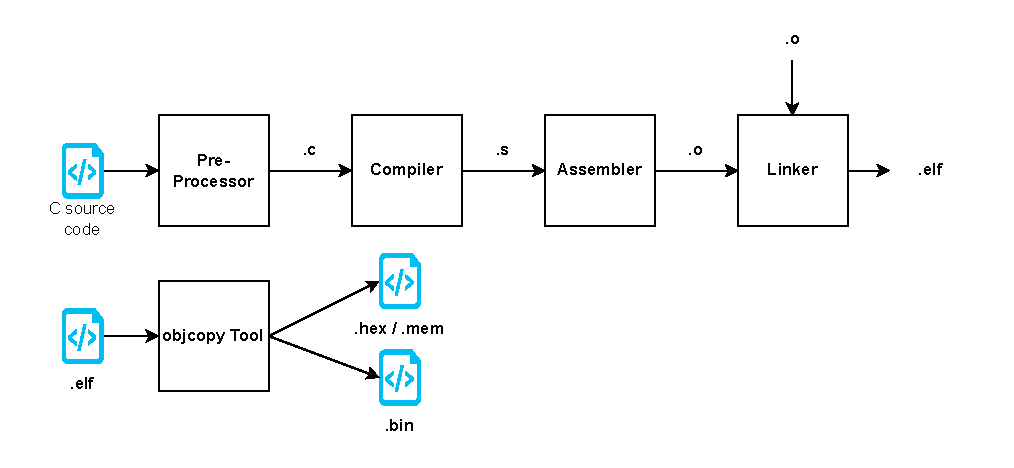
\includegraphics[width=0.9\textwidth]{Thesis_Report/figures/c_to_machine.pdf}
  \caption{Transformation of a C program into machine-executable code.}
  \label{fig:rwu_c_to_machine}
\end{figure}

\begin{enumerate}
  \item \textbf{Preprocessing:}  
  The C preprocessor (\texttt{cpp}) expands all macros, evaluates conditional compilation directives, and includes header files.  
  The result is a pure C file with no preprocessor directives.

  \item \textbf{Compilation:}  
  The compiler (\texttt{gcc}) parses the preprocessed C source and translates it into assembly code for the target instruction set (in this case, RV64I).  
  This stage performs syntax analysis, optimization, and instruction selection based on the chosen compiler flags (\texttt{-O0}–\texttt{-Os}).

  \item \textbf{Assembly:}  
  The assembler (\texttt{as}) converts the assembly file into a relocatable object file (\texttt{.o}).  
  Each object file contains machine instructions and symbol tables describing functions, variables, and section addresses.

  \item \textbf{Linking:}  
  The linker (\texttt{ld}) combines one or more object files and applies the linker script (\texttt{linker.ld}) to assign final memory addresses.  
  It resolves external references and produces an executable file in the ELF (Executable and Linkable Format) structure.

  \item \textbf{Binary Conversion:}  
  The object copy utility (\texttt{objcopy}) extracts the executable sections from the ELF file and converts them into a flat binary or Verilog hex file.  
  For RWU-RV64I, this step produces the \texttt{riscvtest.mem} file that can be directly loaded into the instruction memory of the FPGA or simulation model.
\end{enumerate}



\subsection{Relevance to RWU-RV64I Toolchain}
The RWU-RV64I toolchain replicates this entire process through a single \texttt{Makefile}.  
Each build automatically runs preprocessing, compilation, assembly, linking, and binary conversion, followed by copying the generated memory file into the simulation directory.  
This automation guarantees that the machine code loaded into the RWU-RV64I instruction memory is always synchronized with the C source code and corresponding linker configuration.

\noindent In summary, the process of converting high-level C code into executable instructions ensures that the software toolchain bridges the gap between algorithmic design and hardware execution on the RWU-RV64I platform.


\subsection{Compiler and Assembler}
The GNU Compiler Collection (GCC) translates C source code into assembly instructions compatible with the target processor architecture.  
For RISC-V, the cross-compiler is typically provided as \texttt{riscv64-unknown-elf-gcc}, which produces code conforming to the 64-bit base integer instruction set (RV64I).  
The assembler, part of the GNU Binutils package, then converts this assembly code into relocatable object files ready for linking.

\subsection{Linker and Object Utilities}
The GNU linker (\texttt{ld}) combines object files according to a user-defined memory layout specified in a linker script.  
This script defines how program sections—such as \texttt{.text}, \texttt{.data}, and \texttt{.bss}—are placed within the target’s physical or simulated memory.  
Additional utilities such as \texttt{objcopy} and \texttt{objdump} support binary conversion and inspection, allowing executable images to be adapted for FPGA or simulation-based environments.

The GNU toolchain is widely used in both academia and industry for RISC-V development due to its flexibility, open-source nature, and strong integration with modern IDEs such as Eclipse~\cite{eclipse-cdt,riscv-gnu-toolchain}.
\subsection{Startup and Initialization (crt0.s)}
The startup file (\texttt{crt0.s}) provides the software equivalent of a reset handler.  
When the RWU-RV64I core resets, the program counter begins execution at address \texttt{0x0}, where \texttt{\_start} resides.  
The startup routine performs the following steps:
\begin{enumerate}
  \item Loads the address of \texttt{\_\_stack\_top} and sets the stack pointer (\texttt{sp}).
  \item Clears the \texttt{.bss} section using store instructions.
  \item Calls the user-defined \texttt{main()} function.
  \item Enters an infinite loop if \texttt{main()} returns.
\end{enumerate}
This structure ensures deterministic initialization of memory and registers, comparable in purpose to ARM Cortex-M reset handlers but tailored for the RWU-RV64I’s simpler reset model.

\subsection{Build Automation and Workflow}
The firmware build process is automated using a unified \texttt{Makefile}.  
It automatically detects the single C source file, compiles it, links it with \texttt{crt0.s}, and generates all simulation artifacts.  
The primary build steps are:
\begin{enumerate}
  \item Compilation of C source files into object files.
  \item Linking and generation of the ELF executable.
  \item Conversion of ELF into a Verilog memory image (\texttt{.v}) and binary file (\texttt{.bin}).
  \item Automatic copying of the memory image to the simulation directory for RTL testing.
\end{enumerate}
The toolchain also supports optional waveform simulation and debugging using Vivado’s \texttt{xsim}, allowing verification of instruction flow and GPIO behavior at the signal level.

\section{Program Size Optimization Techniques}
Embedded systems often operate under stringent memory and performance constraints.  
For the RWU-RV64I, only 32~KiB of instruction memory and 8~KiB of data memory are available, making efficient code generation essential.

\subsection{Compiler Optimization Levels}
GCC provides several optimization levels that balance compilation time, execution speed, and code size~\cite{gcc}.  
Common options include:
\begin{itemize}
  \item \texttt{-O0}: No optimization; preserves direct mapping from source to assembly for debugging.
  \item \texttt{-O1}: Enables basic optimizations like constant propagation and dead code elimination.
  \item \texttt{-O2}: Performs aggressive loop and inlining optimizations for performance.
  \item \texttt{-Os}: Optimizes for minimal code size while retaining core performance.
\end{itemize}
In this thesis, the size impact of each level is evaluated using \texttt{riscv64-unknown-elf-size}.

\subsection{Section Placement and Symbol Stripping}
Further reduction in program size can be achieved by stripping unused symbols and debug information using \texttt{objcopy} or \texttt{strip}.  
Additionally, the linker script arranges code and data in memory so that read-only sections reside in IMEM, while writable data and stack occupy DMEM.  
This deliberate separation maximizes usable space and prevents overlap between instruction and data spaces.

\subsection{Harvard Architecture Implications}
The RWU-RV64I implements a strict Harvard architecture where instruction and data memories are physically distinct.  
As a result, the startup code avoids data relocation or copying from IMEM to DMEM.  
All global and static variables are zero-initialized at runtime, and function calls operate directly within the Harvard memory model.  
This separation simplifies memory management, eliminates self-modifying code, and aligns with standard embedded RISC-V design practices.

\section{Related Work}
Numerous research efforts have addressed RISC-V toolchain adaptation and educational core development.  
Waterman and Asanović~\cite{riscv-spec} first outlined the modularity and openness of RISC-V, inspiring subsequent academic implementations.  
SiFive and lowRISC provide reference toolchains that rely on standard libraries such as Newlib~\cite{sifive-toolchain}, whereas the RWU-RV64I setup demonstrates a minimalistic, bare-metal configuration tailored for teaching and FPGA experimentation.  
Similar minimal toolchains have been explored in open-source cores like PicoRV32 and VexRiscv, but most target 32-bit designs with smaller address spaces.  
By contrast, the RWU-RV64I toolchain focuses on a 64-bit environment and precise control over linker and startup behavior, which are often abstracted away in more complex systems.

\section{Summary}
This chapter presented the theoretical and practical background relevant to the RWU-RV64I project.  
It explained the RISC-V RV64I ISA, its programming model, and the components of the bare-metal toolchain.  
Additionally, it described size optimization techniques and summarized related efforts in RISC-V education and research.  
The following chapter provides a detailed overview of the RWU-RV64I hardware system, including its memory architecture, peripherals, and simulation environment.
